\documentclass[letter, 12pt]{article}

\usepackage[margin=0.5in]{geometry}

%equation spacing
\usepackage{xpatch}
\xapptocmd\normalsize{%
 \abovedisplayskip=0pt plus 0pt minus 0pt
 \abovedisplayshortskip=0pt plus 0pt
 \belowdisplayskip=0pt plus 0pt minus 0pt
 \belowdisplayshortskip=0pt plus 0pt minus 0pt
}{}{}

% \usepackage{blindtext}
\usepackage{amssymb,amsfonts,amsmath}

%%%%%%%%%%%%%%%%%%%%%%%%%%%%%%
%% OPTIONAL MACRO FILES
%% Insert self-defined macros here.
%% \newcommand definitions are recommended; \def definitions are supported

\usepackage[pdftex]{graphicx}
\usepackage{amsthm}
\usepackage{textcomp}
\usepackage{latexsym}
\usepackage{enumerate}
\usepackage{natbib}

\newtheorem{thm}{Theorem}[section]
\newtheorem{cor}[thm]{Corollary}
\newtheorem{ex}[thm]{Example}
\newtheorem{conj}[thm]{Conjecture}
\newtheorem{prob}[thm]{Problem}
\newtheorem{lem}[thm]{Lemma}
\newtheorem{prop}[thm]{Proposition}
\theoremstyle{definition}
\newtheorem{defn}[thm]{Definition}
\theoremstyle{remark}
\newtheorem{rem}[thm]{Remark}
%\numberwithin{equation}{section}

\newcommand{\set}[1]{\lbrace #1 \rbrace}
\newcommand{\setc}[2]{\lbrace #1 \mid #2 \rbrace}
\newcommand{\vv}[1]{{\mathbf{#1}}}
\newcommand{\dd}{{\mathrm{d}}}
\newcommand{\pd}[2]{\frac{\partial #1}{\partial #2}}
\newcommand{\pdn}[3]{\frac{\partial^#1 #2}{\partial #3^#1}}
\newcommand{\od}[2]{\frac{\dd #1}{\dd #2}}
\newcommand{\odn}[3]{\frac{\dd^#1 #2}{\dd #3^#1}}
\newcommand{\avg}[1]{\left< #1 \right>}

%--- operators
\DeclareMathOperator{\trop}{trop}
\DeclareMathOperator{\adj}{adj}
\DeclareMathOperator{\tr}{tr}
\DeclareMathOperator*{\argmax}{argmax}
\DeclareMathOperator{\Var}{Var}

\newcommand{\mb}{\mathbf}
\newcommand{\argmin}{\operatornamewithlimits{argmin}}
\newcommand{\doublebar}{\bigl|\!\bigr|}

% Default fixed font does not support bold face
\DeclareFixedFont{\ttb}{T1}{txtt}{bx}{n}{12} % for bold
\DeclareFixedFont{\ttm}{T1}{txtt}{m}{n}{12}  % for normal

% Custom colors
\usepackage{color}
\definecolor{deepblue}{rgb}{0,0,0.5}
\definecolor{deepred}{rgb}{0.6,0,0}
\definecolor{deepgreen}{rgb}{0,0.5,0}

\usepackage{listings}

% Python style for highlighting
\newcommand\pythonstyle{\lstset{
language=Python,
basicstyle=\ttm,
otherkeywords={self},             % Add keywords here
keywordstyle=\ttb\color{deepblue},
emph={},          % Custom highlighting
emphstyle=\ttb\color{deepred},    % Custom highlighting style
stringstyle=\color{deepgreen},
%frame= tb,                         % Any extra options here
showstringspaces=false            % 
}}


% Python environment
\lstnewenvironment{python}[1][]
{
\pythonstyle
\lstset{#1}
}
{}

% Python for external files
\newcommand\pythonexternal[2][]{{
\pythonstyle
\lstinputlisting[#1]{#2}}}

% Python for inline
\newcommand\pythoninline[1]{{\pythonstyle\lstinline!#1!}}


\newcommand{\commentfe}[1]{{\color{red}FE: #1}}

\begin{document}

\title{Starter Manual for HDNET in Python}
\author{\normalsize Christopher Hillar, Redwood Center for Theoretical Neuroscience, Berkeley, CA 94720\\
\normalsize Felix Effenberger, Max-Planck-Institute for Mathematics in the Sciences, Leipzig, Germany
}
\date{}

\pagenumbering{gobble}


\maketitle



\textbf{Introduction}.  Here, we describe the basic functionality of the HDNET library in Python
\begin{center}
\texttt{https://github.com/qualiaphile/hdnet.git} \\
\end{center}

For demonstration purposes we will work with a synthetic data set in the following. Spiking activity of 10 hypothetical cells are assumed to be given as iid. Poisson processes. Upon binning with a given bin width, this yields Bernoulli processes in discrete time. We create such Bernoulli data and then insert hypothetical correlations by means of a number of co-activations of different cell groups (also known as cell assemblies).

We first import the necessary modules into our Python session (we recommend using ipython in pylab mode, i.e. running \texttt{ipython --pylab} to paste and run text copied to the clipboard from this tutorial using the magic command \texttt{\%paste}).

\begin{python}
import numpy as np
import matplotlib.pyplot as plt
from hdnet.spikes import Spikes
from hdnet.spikes_,model import SpikeModel, BernoulliHomogeneous, \ 	
	DichotomizedGaussian
\end{python}

We create two trials of $200$ time bins of spikes from $10$ neurons.

\begin{python}
spikes_arr = (np.random.random((2, 10, 200)) < .05).astype(int)
spikes_arr[0, [1, 5], ::5] = 1 # insert correlations
spikes_arr[1, [2, 3, 6], ::11] = 1  # insert correlations
spikes = Spikes(spikes_arr=spikes_arr)
\end{python}

We can now plot a raster of the trials and covariances:

\begin{python}
plt.figure()
plt.title('Raw spikes')}
plt.matshow(spikes.rasterize(), cmap='gray')} 

plt.figure()
plt.title('Raw spikes covariance')
plt.matshow(spikes.covariance().reshape((2 * 10, 10)), cmap='gray')}

plt.show()
\end{python}

Next, we would like to model this noisy binary data.   First, we try to model each trial with a separate i.i.d. Bernoulli random binary vector having the same neuron means as in each trial:

\begin{python}
spike_model = BernoulliHomogeneous(spikes=spikes)
BH_sample_spikes = spike_model.sample_from_model()

plt.figure()
plt.title('BernoulliHomogeneous sample')
plt.matshow(BH_sample_spikes.rasterize(), cmap='gray')

plt.figure()
plt.title('BernoulliHomogeneous covariance')
plt.matshow(BH_sample_spikes.covariance().reshape((2 * 10, 10)), cmap='gray')

plt.show()
\end{python}

As we can see in Fig.~\ref{fake_ex_fig}, the samples from Bernoulli have the correct firing rates in each trial, but not the coordinated aspect (as can be seen in the covariance matrices for each trial, which are basically diagonal matrices).   A better model that keeps track of the correlations is the Dichotomized Gaussian \cite{bethge2008}: \\

\begin{python}
spike_model = DichotomizedGaussian(spikes=spikes)

DG_sample_spikes = spike_model.sample_from_model()

plt.figure()
plt.title('DichotomizedGaussian sample')
plt.matshow(DG_sample_spikes.rasterize(), cmap='gray')

plt.figure()
plt.matshow(DG_sample_spikes.covariance().reshape((2 * 10, 10)), cmap='gray')
plt.title('DichotomizedGaussian covariance')

plt.show()
\end{python}

Finally, we try and model the data with a Hopfield network trained using MPF over all the trials:

\begin{python}
spike_model = SpikeModel(spikes=spikes)
spike_model.fit()  # note: this fits a single network to all trials
spike_model.chomp()

converged_spikes = Spikes(spikes_arr=spike_model.hopfield_spikes_arr)

plt.figure()
plt.title('Converge dynamics on Raw data')
plt.matshow(converged_spikes.rasterize(), cmap='gray')

plt.figure()
plt.title('Covariance of converged memories')
plt.matshow(converged_spikes.covariance().reshape((2 * 10, 10)), cmap='gray')

plt.show()
\end{python}
 
\begin{figure}
\begin{center}
\textbf{a)}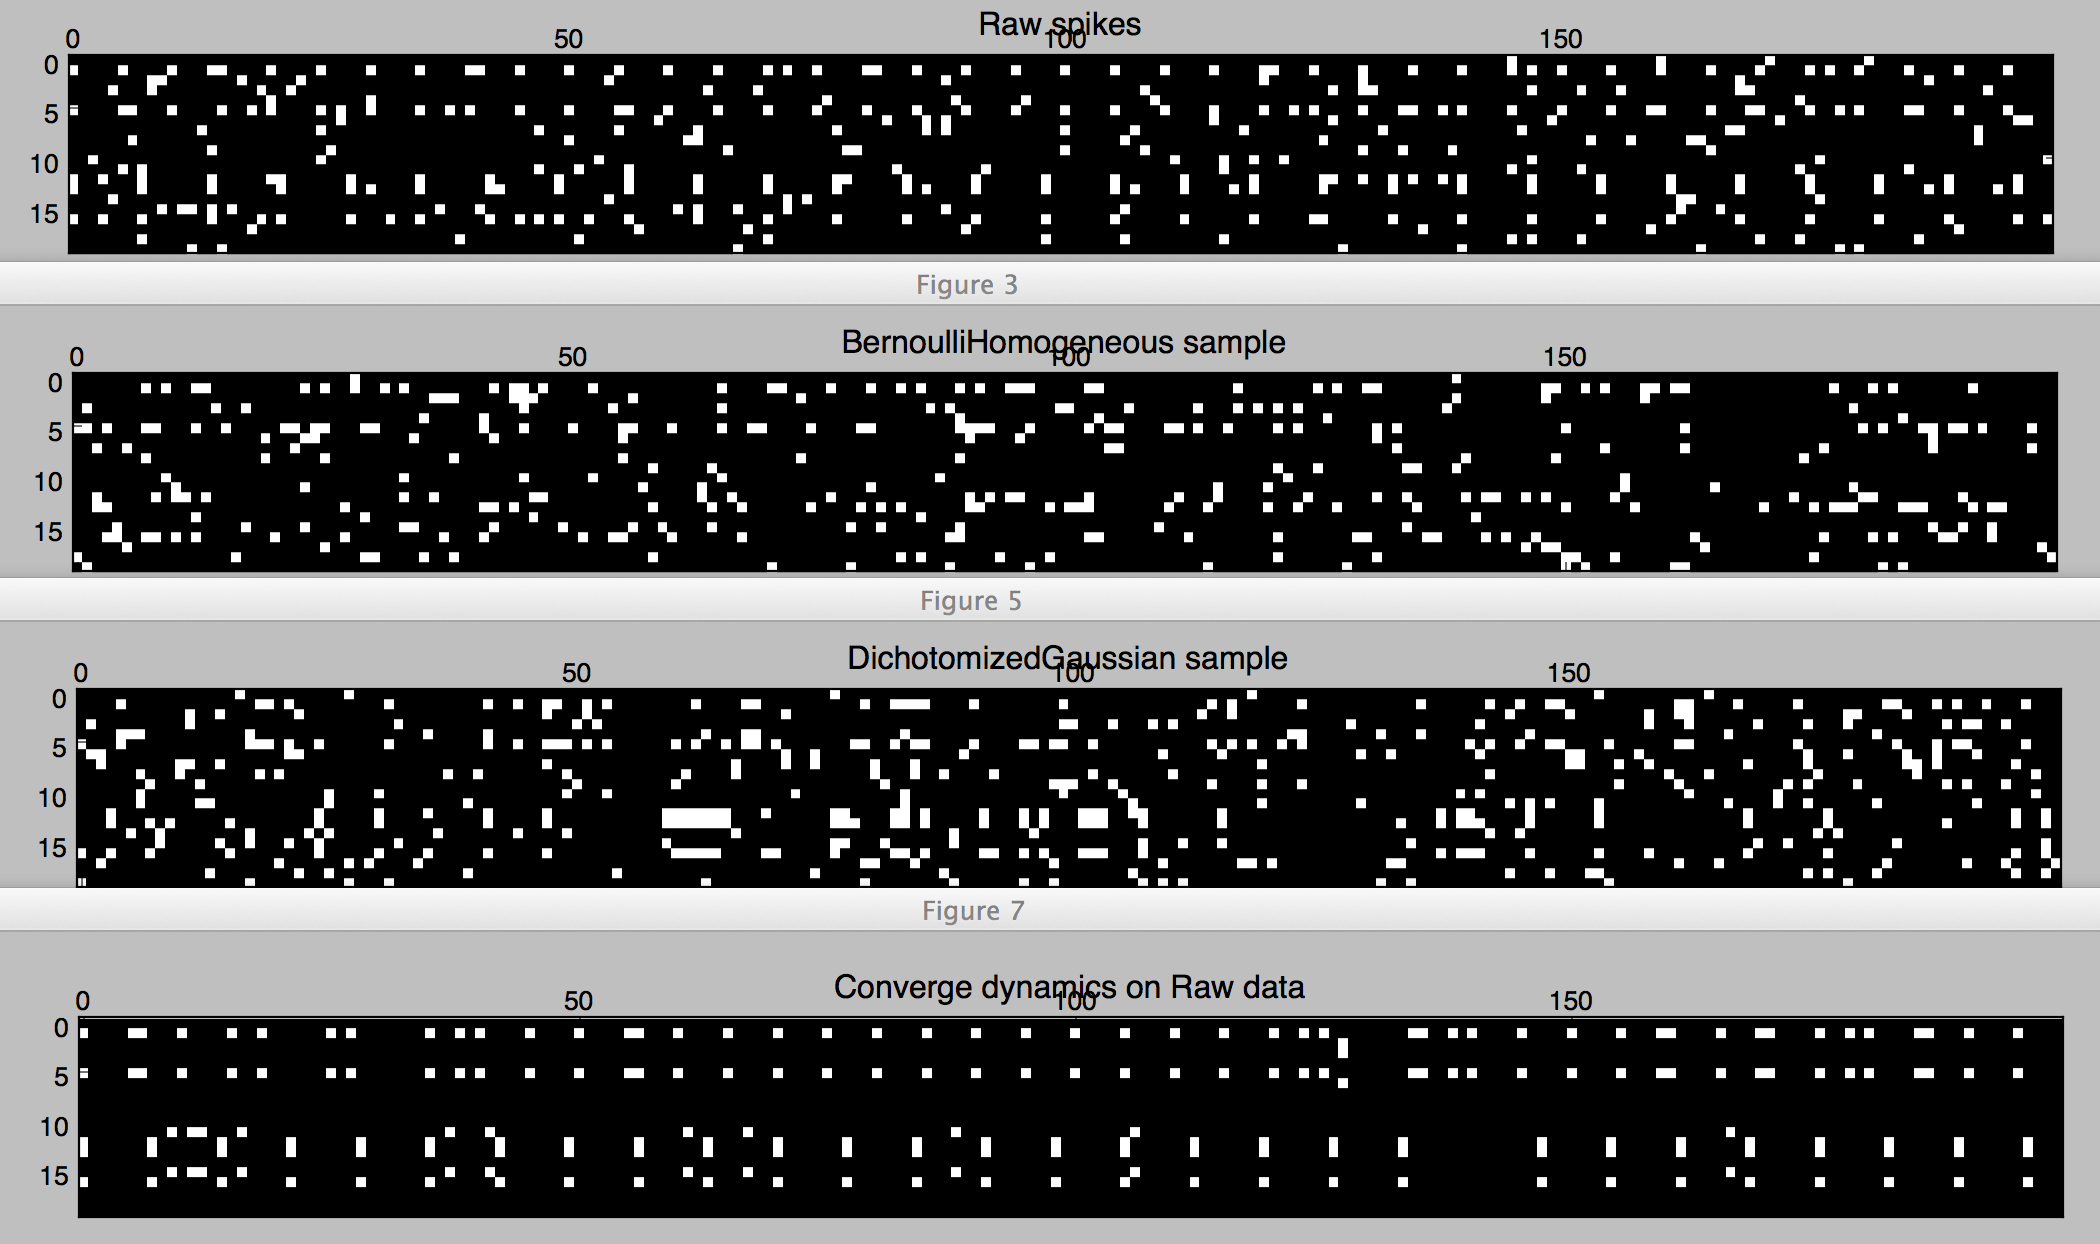
\includegraphics[width=.41\linewidth]{demo_fake_spikes.png} 
\textbf{b)}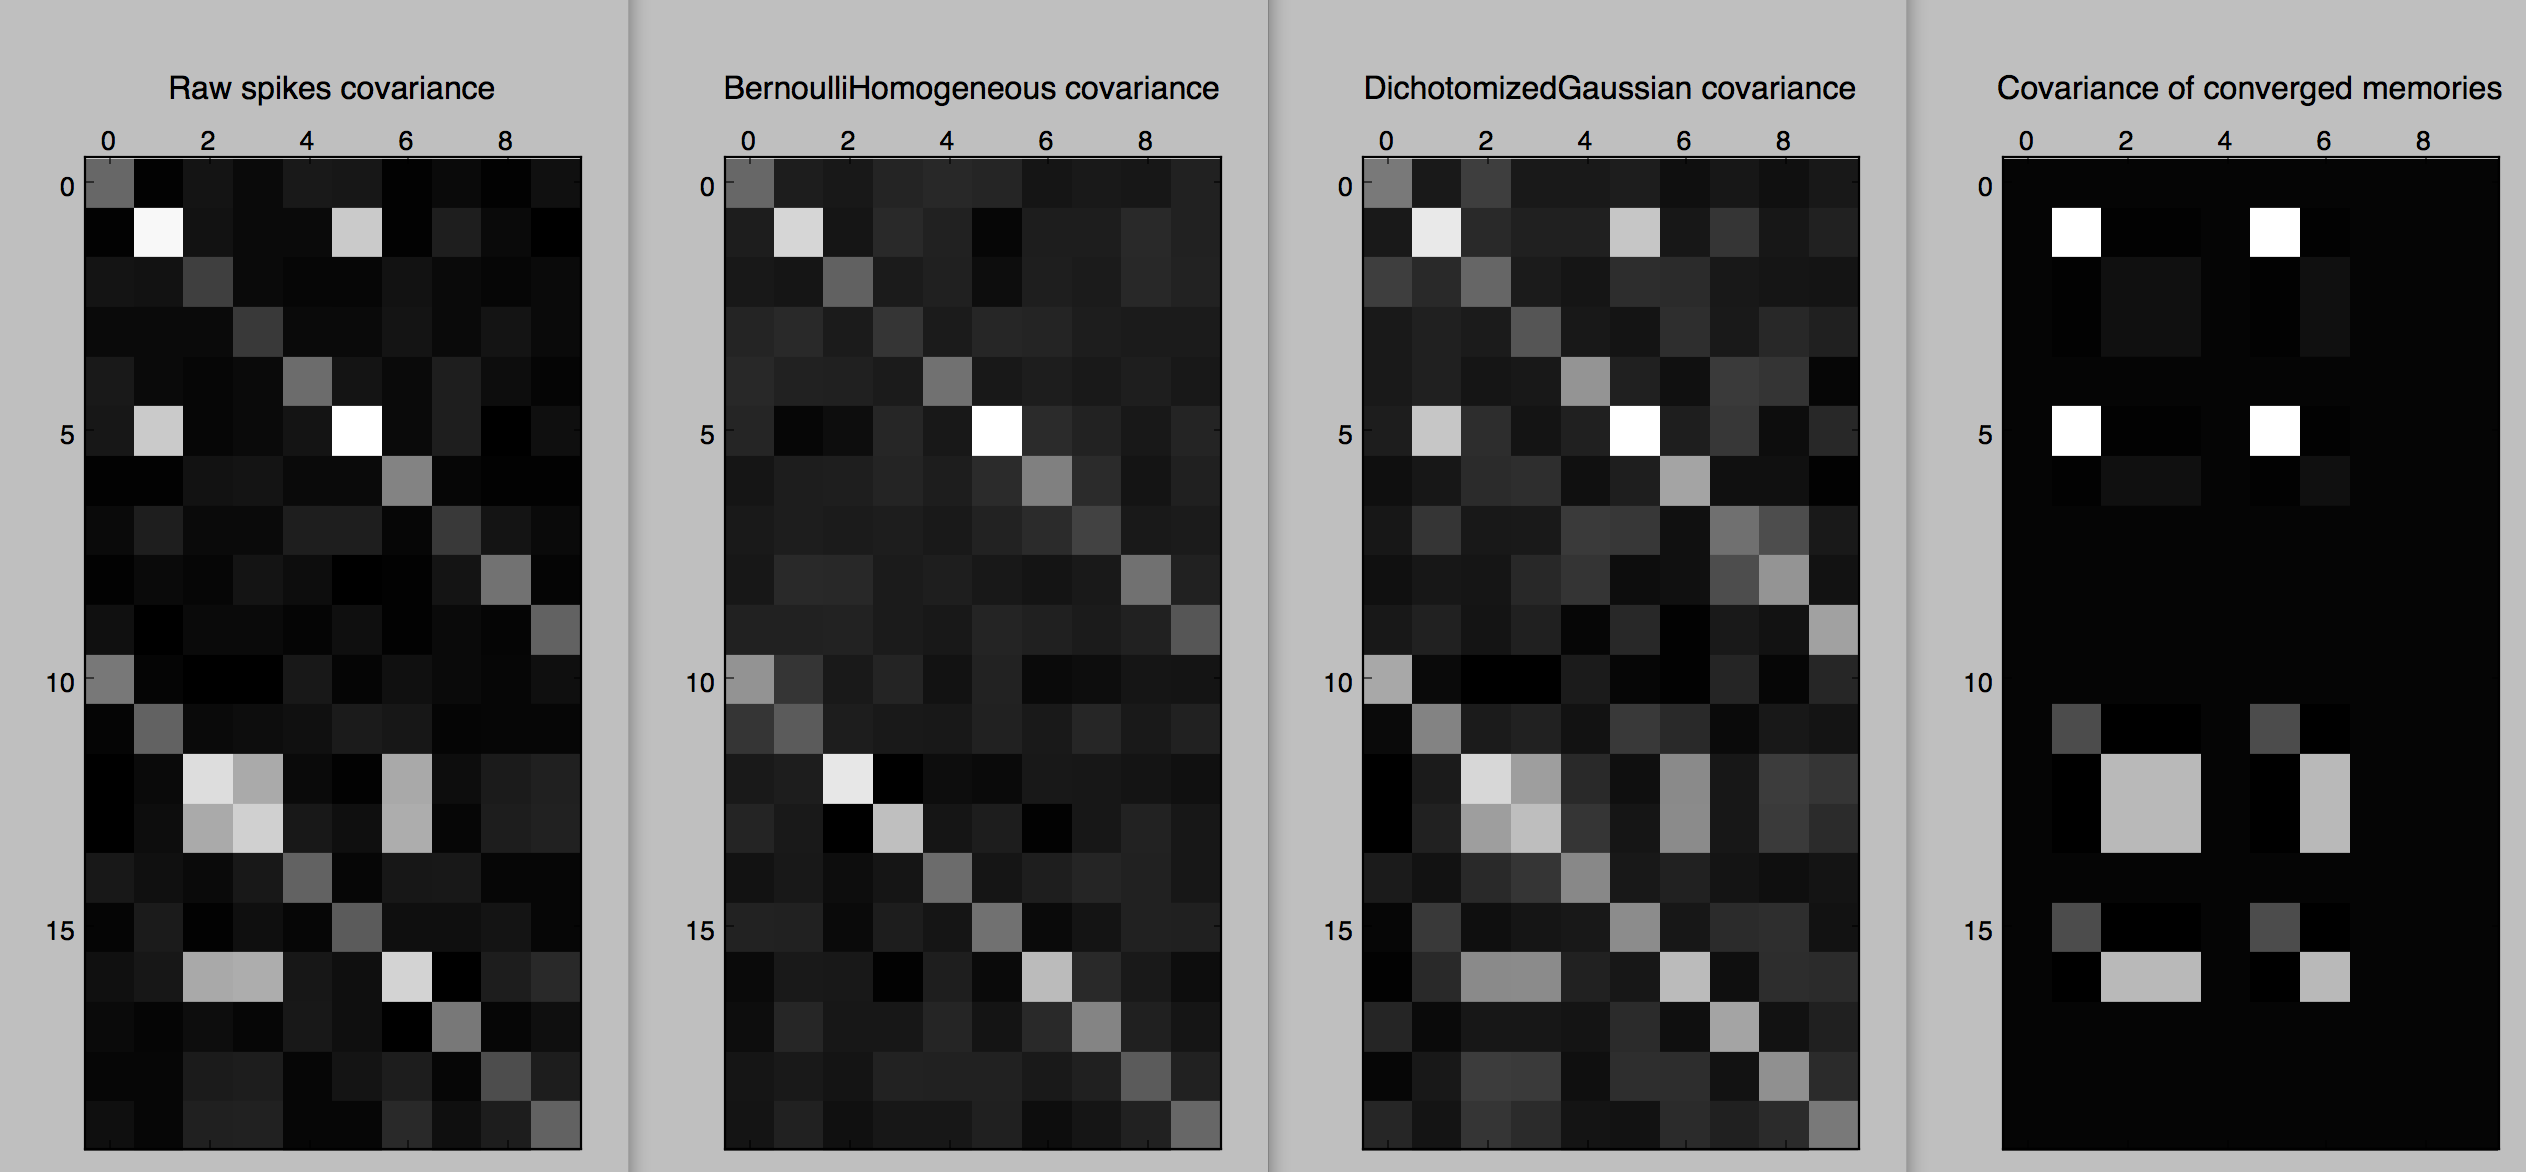
\includegraphics[width=.53\linewidth]{cov_demo.png} 
\caption{\textbf{Fake data example}. Two trials with 10 neurons.}
\label{fake_ex_fig}
\vspace{-.8cm}
\end{center}
\end{figure}

\textbf{More advanced features}.  One thing we would like to do is examine the structure of the memories:

\begin{python}
# plot memory label (its chronological appearance) as a function of time
plt.figure()
plt.scatter(range(len(spike_model.memories.sequence)),
		1 + np.array(spike_model.memories.sequence))
plt.xlabel('time bin')
plt.ylabel('Memory number (chronological order of appearance)')
plt.title('Converged memory label at each time bin')

# versus the raw data
plt.figure()
plt.scatter(range(len(spike_model.emperical.sequence)),
		1 + np.array(spike_model.emperical.sequence))
plt.ylabel('Raw pattern number (chronological order of appearance)')
plt.xlabel('time bin')
plt.title('Raw pattern label at each time bin')

plt.show()
\end{python}
 
Notice in Fig.~\ref{fake_ex_fig2} that the converged dynamics of the trained Hopfield networks on the original data does reveal the 
hidden assemblies for the most part.

\begin{figure}[t!]
\begin{center}
\textbf{a)}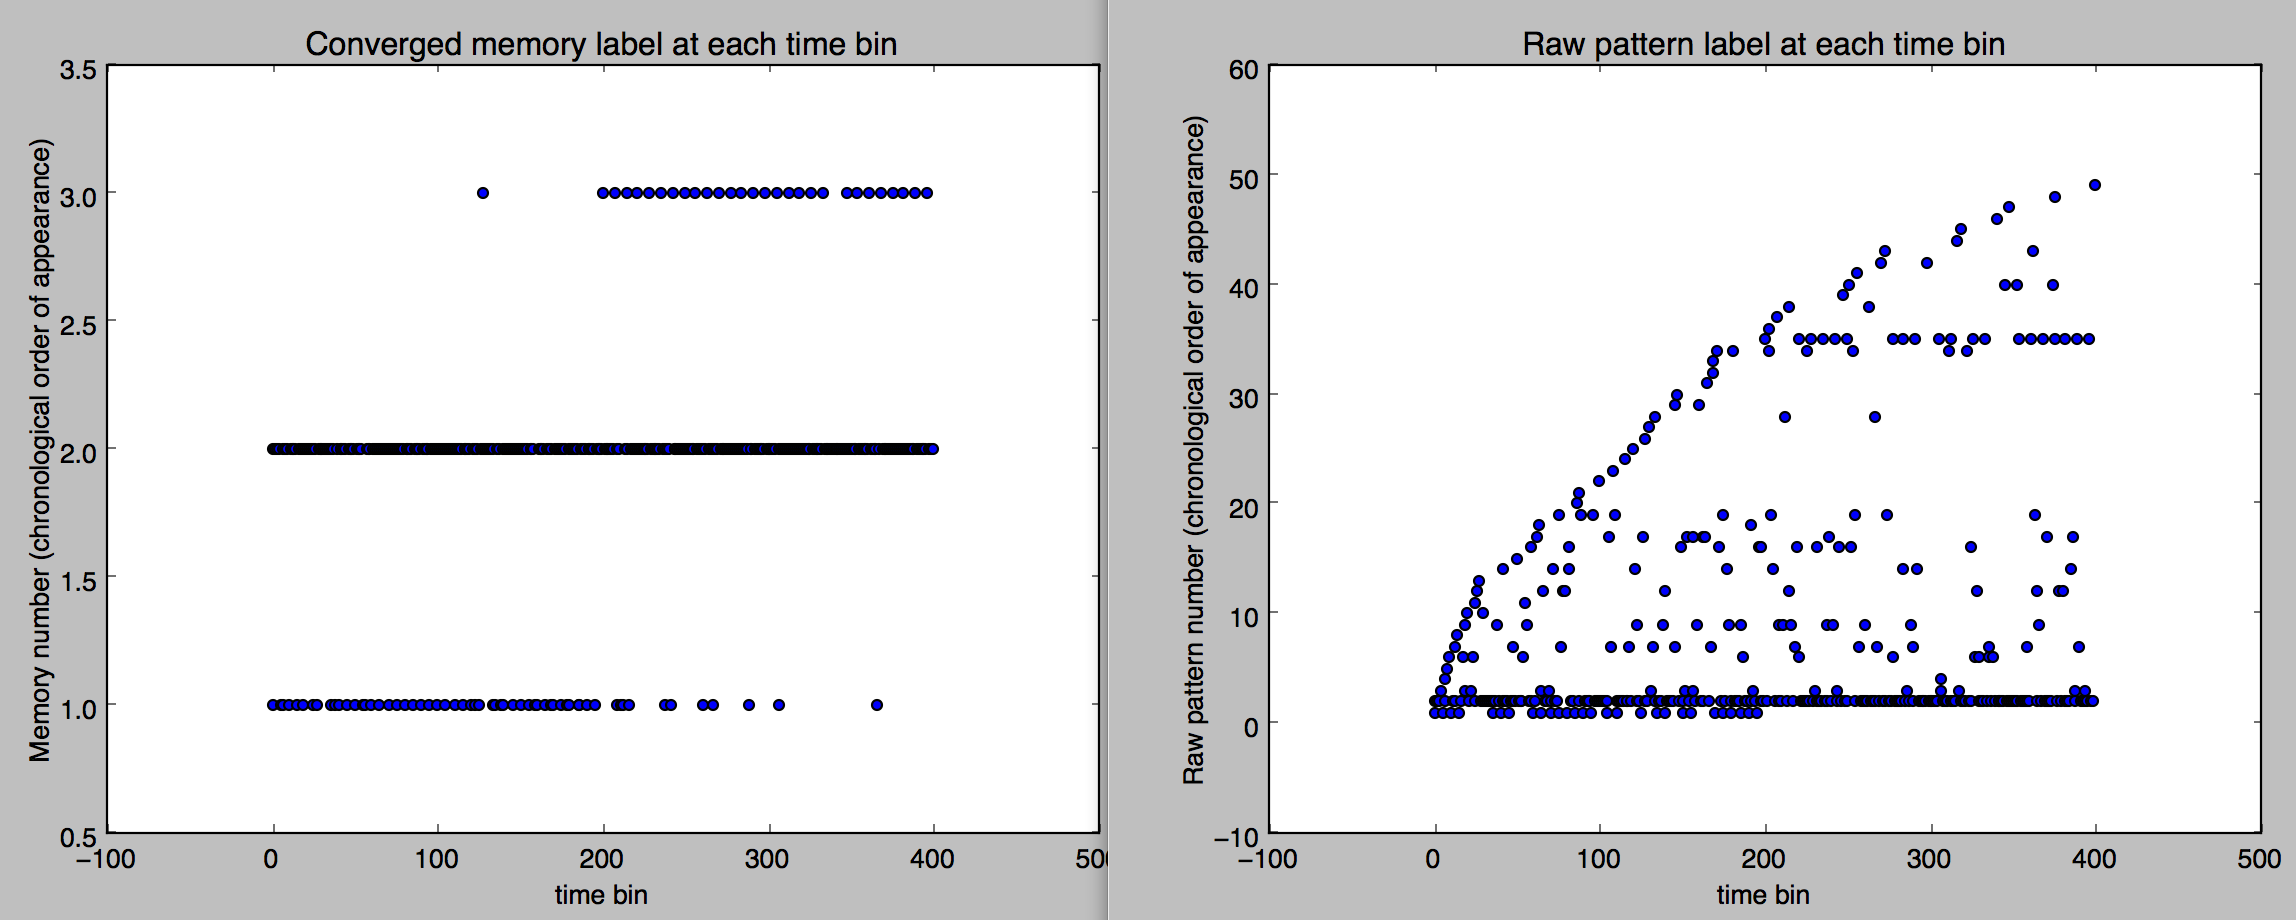
\includegraphics[width=.75\linewidth]{chron_order_patterns.png} 
%\textbf{b)}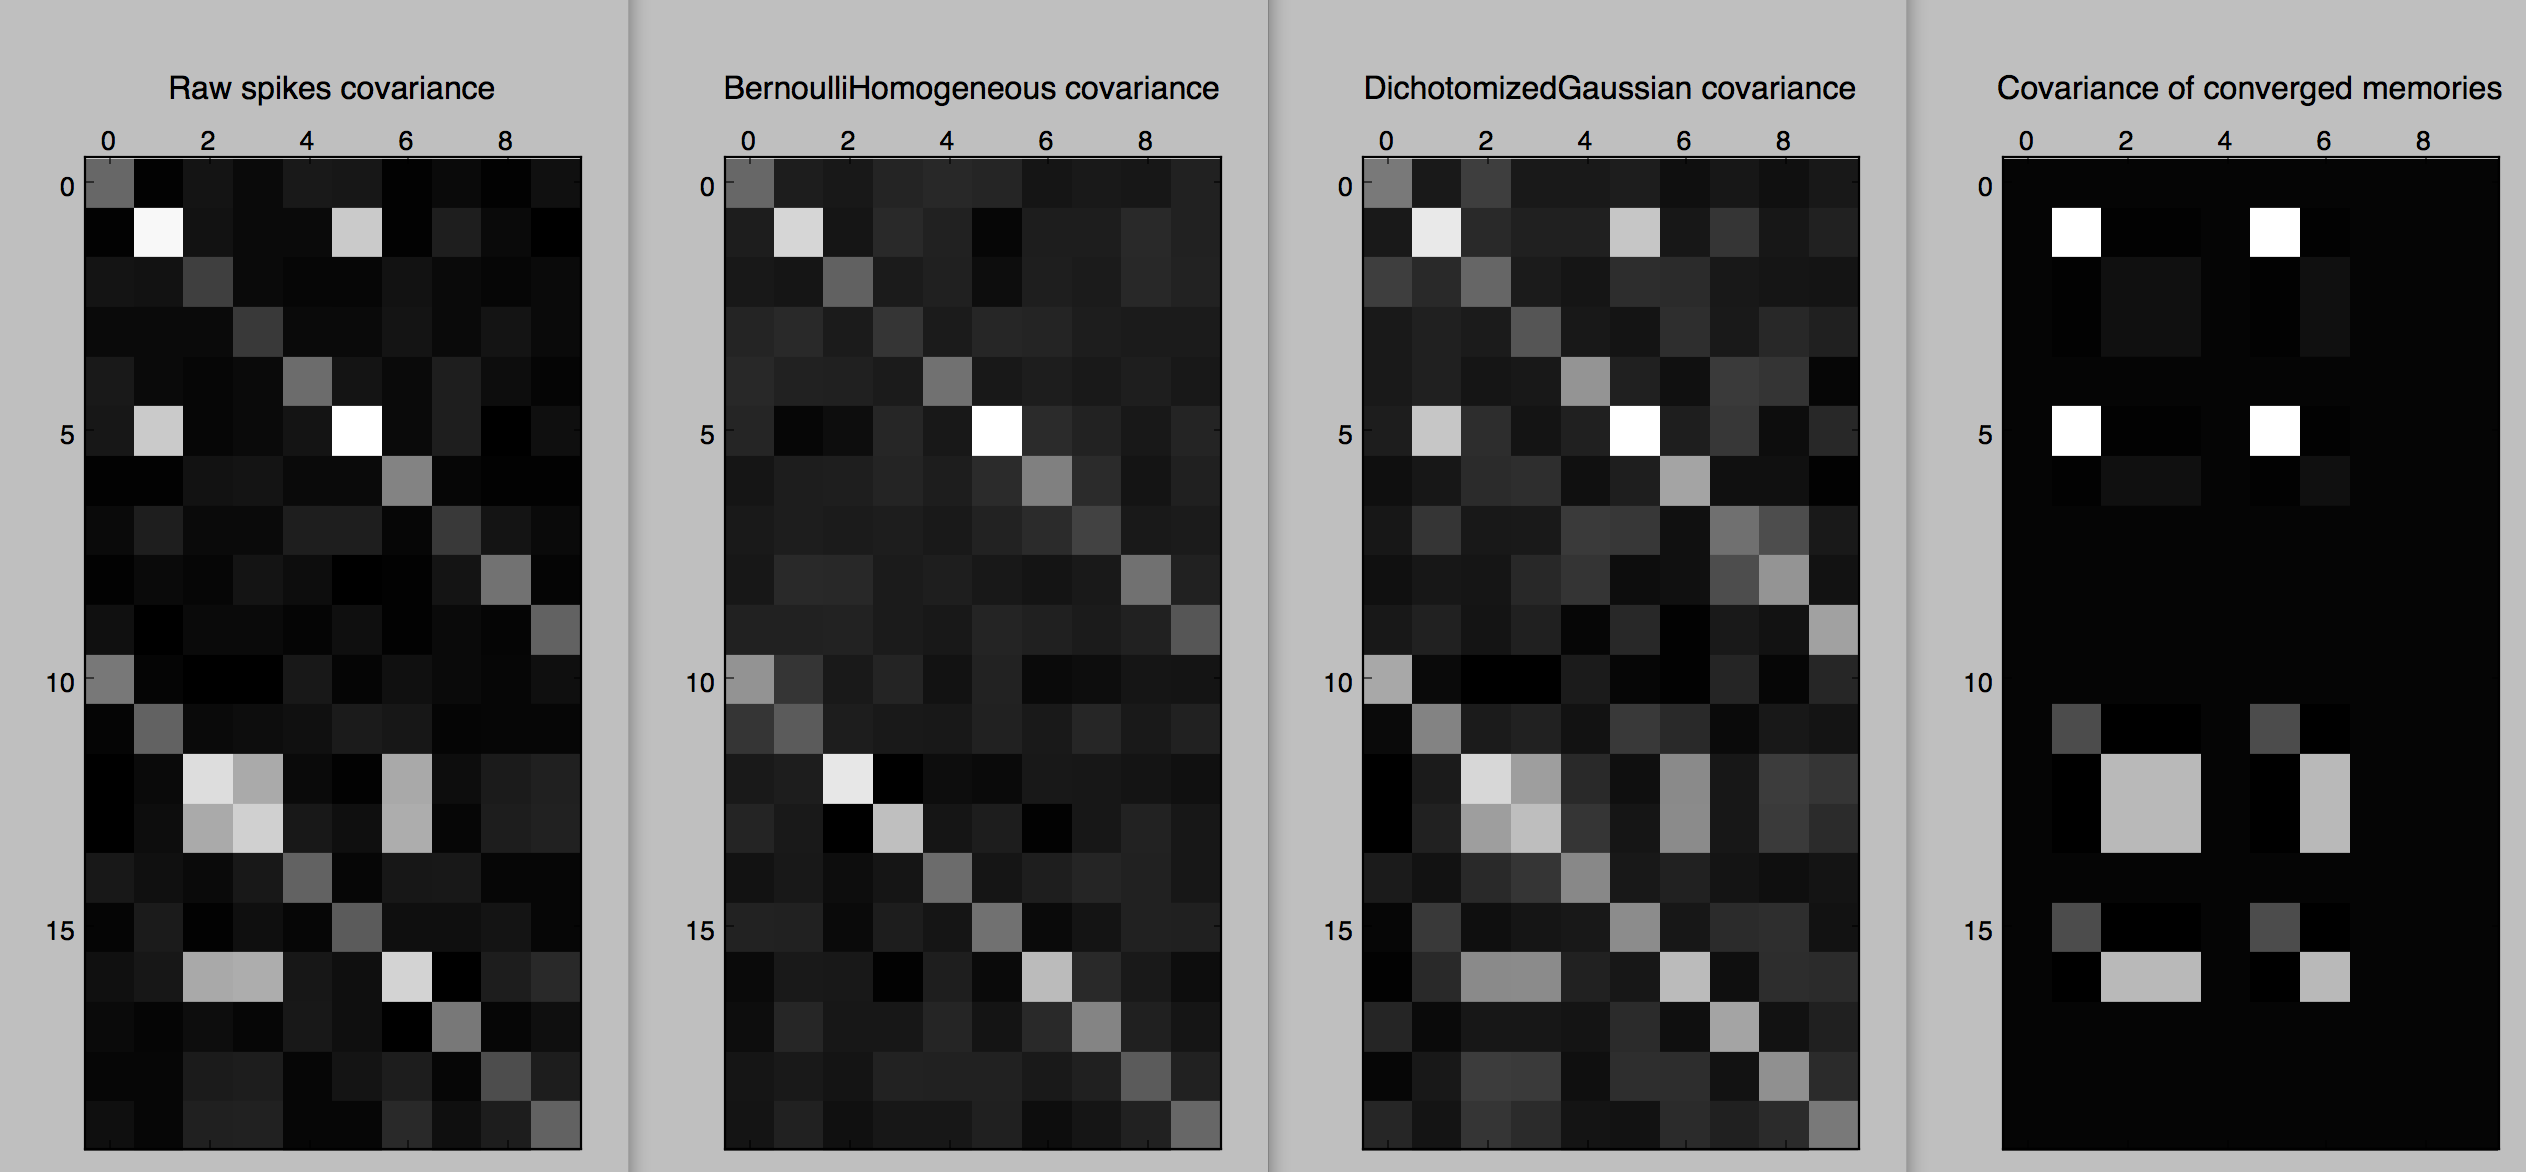
\includegraphics[width=.53\linewidth]{cov_demo.png} 
\textbf{b)}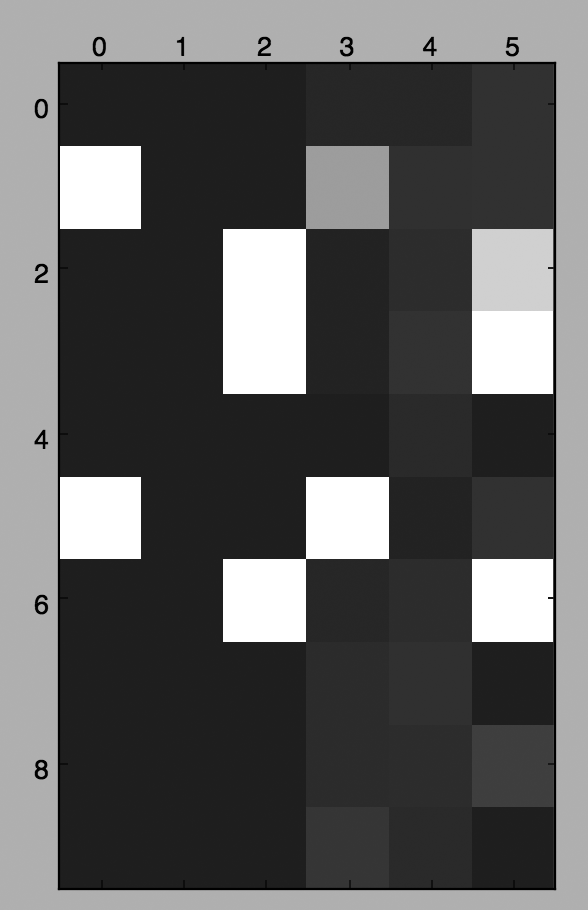
\includegraphics[width=.19\linewidth]{memories_stas.png} 
\caption{\textbf{Continuing fake data example}. \textbf{a)} Patterns (Converged at left, Raw on right) over time bins labeled on the $y$-axis by their first appearance in the dataset.  \textbf{b)}  Memories in network (left) and Memory Triggered Averages (at right).}
\label{fake_ex_fig2}
\vspace{-.8cm}
\end{center}
\end{figure}

Now that we know there are basically two assemblies, one showing up lots in the first trial and the other in the second.  Let's look at the
memories and their corresponding MTA's (\textit{memory triggered averages}).  The code below generates Fig.~\ref{fake_ex_fig2}\textbf{b}, which displays
a matrix whose first 3 columns are the memories in the network and whose next 3 columns are the average of Raw data patterns converging to the corresponding memory in the first 3 columns.

\begin{python}
# memories are ordered by their first appearance
bin_memories = spike_model.memories.fp_list
arr = np.zeros((spike_model.original_spikes.N, 2 * len(bin_memories)))
for c, memory in enumerate(bin_memories):
	arr[:, c] = spike_model.memories.fp_to_binary_matrix(c)

for c, memory in enumerate(bin_memories):
	arr[:, c + len(bin_memories)] = spike_model.memories.stas[memory] /
			spike_model.memories.counts[memory]

print "Probabilities of each memory:"
print zip(bin_memories, spike_model.memories.to_prob_vect())
\end{python}

\textbf{Saving}.  One can save Learners and Memories.

\scriptsize
\setlength{\bibsep}{0pt plus 0.3ex}
\bibliographystyle{abbrv}
\bibliography{hdnet_manual} 

\end{document}
